\documentclass[12pt, titlepage]{article}
\usepackage[ngerman]{babel}
\usepackage[utf8]{inputenc}
\usepackage{color}
\usepackage[a4paper, lmargin={3cm}, rmargin={2.5cm}, tmargin={3cm}, bmargin={2cm}]{geometry}
\usepackage{amssymb}
\usepackage{amsthm}
\usepackage{graphicx}
\usepackage{helvet}
\usepackage{microtype}
\usepackage{setspace}
\usepackage{csquotes}
\usepackage{xpatch}
\usepackage{comment}
\usepackage[backend=biber, %% Hilfsprogramm "biber" (statt "biblatex" oder "bibtex")
style=authoryear-ibid, %% Zitierstil (siehe Dokumentation)
natbib=true, %% Bereitstellen von natbib-kompatiblen Zitierkommandos
hyperref=false, %% hyperref-Paket verwenden, um Links zu erstellen
ibidpage=true
]{biblatex}
\addbibresource{literatur.bib}

\renewcommand{\familydefault}{\sfdefault}
\setlength\parindent{0pt}


\begin{document}
% Leere Titelseite
\pagenumbering{gobble}
\newpage\null\thispagestyle{empty}\newpage

\begin{titlepage}
    \normalsize{Hochschule Hannover, Fakultät IV: Wirtschaft und Informatik

    Bachelorarbeit im Studiengang Wirtschaftsinformatik, Wintersemester 2021/2022} 
    
    \sloppy 
    \textbf{\Large{\\Konzeption, Datenmodellierung und prototypischer Aufbau eines Prozess-Tracking-Tools zur Steuerung und Umsetzungsverfolgung einer S/4HANA Transformation im Vorgehensmodell eines IT-Beratungsunternehmens}}
    \vspace{10cm}
    \normalsize{\\Abgabedatum: 08. Februar 2022 \vspace{1cm}\\Lukas Hampel\\Matrikelnummer: 1481025\\Scharnhorststr. 8\\31785 Hameln\vspace{1cm}\\Erstprüfer: Herr Prof. Dr. Raymond Fleck\\Zweitprüfer: Herr Michael Bloß, adesso orange AG}
\end{titlepage}


\section*{Sperrvermerk}
Lorem
\newpage


\pagenumbering{Roman}
\setcounter{page}{3}
\section*{Vorbemerkung}

\newpage

\tableofcontents

\newpage

\section*{Glossar / Abkürzungsverzeichnis}

\newpage

\listoffigures{}
\listoftables{}

\newpage

\section*{Kurzfassung}

\newpage

\pagenumbering{arabic}
\setcounter{page}{1}
\begin{normalsize}
\linespread{1.5}

%Einleitung
\doublespacing
\section{Einleitung}
\subsection{Motivation}
Die SAP SE (fortan, in Abgrenzung zum Produkt, als \glqq{}die\grqq{} SAP bezeichnet) ist der größte Anbieter für Unternehmenssoftware in Europa und hat mit dem Produkt SAP-ERP eine der am weitesten verbreiteten Enterprise-Ressource-Planning (ERP)-Software geschaffen. \\Mit der neusten Generation SAP S/4HANA sollen in den nächsten Jahren die bereits etablierten Versionen SAP R/2 und SAP R/3 sukzessive abgelöst werden, bevor die Unterstützung, in Form von Weiterentwicklungen und Aktualisierungen, durch die SAP im Jahr 2030 vollständig eingestellt wird. Die Generation S/4HANA bringt viele neue Funktionen, unter anderem viele Cloud-Funktionalitäten mit sich, weshalb die Umstellung für die meisten Unternehmen eine große Hürde darstellt, die in der Regel nicht mit den intern vorhandenen Ressourcen bewältigt werden kann. Allerdings bringt die Aktualisierung auf die neuste Generation auch viele Chancen mit sich, um den Aufbau der Systeme und der darin abgebildeten Geschäftsprozesse komplett neu zu denken, 
%NICHT SCHÖN!!!!
da vieles bei der Umstellung sowieso angefasst werden muss. Das erleichtert bspw. die Trennung von historisch gewachsenen Strukturen und die Annäherung bzw. Etablierung des Industriestandards und dessen Best-Practises. Dadurch werden im Anschluss die Wartungskosten für die Systeme verringert und eine Optimierung und Effizienzsteigerung der Geschäftsprozesse erreicht.\\ Um eine solche Transformation durchzuführen, ist jedoch viel Wissen und Erfahrung im Projektmanagement und der Projektorganisation notwendig, vorallem aber auch viel Expertise in den Disziplinen der einzelnen Fachbereiche.
Die SAP setzt in den Bereichen Vertrieb, Service, Betrieb und  Entwicklung ihrer Produkte auf ein breit aufgestelltes Partnerprogramm, in dem Drittunternehmen aufgenommen werden können, um sich für eine Kooperation zu qualifizieren. Dadurch haben sich viele IT-Beratungsunternehmen auf das Themengebiet SAP spezialisiert und bieten nun auch eine SAP S/4HANA-Transformation für ihre Kunden an.

\subsection{Zielsetzung}
In der hier vorliegenden Bachelorarbeit aus dem Studiengang der Wirtschaftsinformatik soll es um die Konzeption, Datenmodellierung und den protypischen Aufbau eines Prozess-Tracking-Tools gehen, das im Vorgehensmodell eines IT-Beratungsunterneh- mens zur SAP S/4HANA-Transformation zum Einsatz kommen soll.\\ 
Das Tool soll auf dem gesamten Transformationspfad in einem S/4HANA-Projekt produktiv zum Einsatz kommen und frühzeitig einen 
Überblick über alle betroffene Transformationsobjekte wiedergeben. 
%nicht schön
Dadurch soll erreicht werden, dass zu jedem Zeitpunkt der aktuelle Fortschritt der Transformation im jeweiligen Prozess wiedergegeben werden kann und kein Artefakt außer acht gelassen wird, wodurch Probleme im späteren Projektverlauf vermieden werden sollen, indem stets alle Aspekte betrachtet werden können.



%Grundlagen
\section{Grundlagen}
Im folgenden Kapitel werden die theoretischen Grundlagen behandelt, die für das Verständnis dieser Arbeit notwendig sind. Dabei geht es in erster Linie um allgemeine Begrifflichkeiten aus dem wirtschaftlichen Kontext des zu entwickelnen Programms.

\subsection{ERP-Systeme}
ERP ist ein Akronym für den englischen Begriff \glqq{}Enterprise Ressource Planning\grqq{}, also das Planen von Unternehmensressourcen, u.a. in den Bereichen Beschaffung, Produktion, Vertrieb, Personalwirtschaft und Finanzwesen. \footcite[Vgl.][523]{wibuch} Ein ERP-System beschreibt somit eine Software, die Prozesse aus diesen Bereichen in einem Anwendungspaket integriert und die dabei anfallenden Daten in einer zentralen Datenbank abspeichert. Dadurch werden Redundanzen in der Datenhaltung vermieden und die Umsetzung von bereichsübergreifenden Unternehmensprozessen ermöglicht \footcite[Vgl.][523]{wibuch}. ERP-Systeme nutzen in der Regel eine Client-Server-Architektur und sind komponentenorientiert, das heißt, Unternehmen können, je nach Anforderungen ihrer Wertschöpfungsprozesse, die benötigten Komponenten frei wählen. Dadurch ist eine schrittweise Einführung der ERP-Software, über einen längeren Zeitraum, möglich. \footcite[Vgl.][524 f.]{wibuch}

\subsection{SAP}
\subsubsection{Die SAP SE}
Die SAP SE wurde im Jahr 1972 von fünf ehemaligen IBM-Mitarbeitern unter dem Namen \glqq{}\underline{S}ystem\underline{a}nalyse und \underline{P}rogrammentwicklung GbR\grqq{}\footcite[Vgl.][]{think-ing}  mit dem Ziel gegründet, eine Standardanwendungssoftware für die Echtzeitverarbeitung zu entwickeln.  Im Jahr 1973 wurde durch die SAP mit dem \glqq{}System RF\grqq{} das erste Produkt für die Finanzbuchhaltung vorgestellt, was den Grundstein für die erste SAP-Generation \glqq{}SAP R/1\grqq{} legen sollte. Durch die ständigen Weiterentwicklungen wurde das System stets erweitert und fand bei immer mehr Kunden anklang. 1976 wurde die Gesellschaft bürgerlichen Rechts aufeglöst und in eine GmbH überführt. Im selben Jahr wurde bereits mit nur 25 Mitarbeitern ein Umsatz von 3,81 Mio. DM erzielt. \footcite[Vgl.][]{sap-fruehejahre}\\Im Jahr 1979 folgt schließlich die zweite Produktgeneration \glqq{}SAP R/2\grqq{}, die eine höhere Stabilität mit sich brachte und in weitere Geschäftsbereiche vordrang. In der Generation R/2 waren bereits die Module RF für Finanzbuchhaltung, RK für die Kostenrechnung, RM für Materialwirtschaft, Produktionsplanung und Instandhaltung, RP für die Personalwirtschaft und RV für den Vertrieb verfügbar.\footcite[Vgl.][]{bewerbungsratgeber}\\Im Jahr 1988 wurde die SAP GmbH schließlich in eine Aktiengesellschaft überführt und startete an der Börse Frankfurt sowie in Stuttgart. Im selben Jahr erwirtschaftetet SAP bereits einen Umsatz von 245 Mio. DM und hatte bereits 940 Mitarbeiter. Bereits zu diesem Zeitpunkt war die dritte Generation \glqq{}SAP R/3\grqq{} in Entwicklung, die schließlich im Jahr 1992 erschien und, in Gegensatz zu ihren Vorgängern, auf einer Client-Server-Architektur aufgebaut war. Das führte dazu, dass SAP immer erfolgreicher wurde und auch international immer weiter expandierte, sodass im Jahr 1997 schließlich 1,6 Mrd. DM  Umsatz erwirtschaftet wurden. 1995 begann SAP damit, seine Vertriebsaktivitäten im deutschen Mittelstand auszubauen, da zuvor die Hauptkundenzielgruppe nur größere Unternehmen waren. In den darauffolgenden Jahren startete die SAP zusammen mit Microsoft seine Internetstrategie und setzte mit \glqq{}mySAP.com\grqq{} vermehrt den Fokus auf E-Commerce und E-Business-Lösungen und seit dem Jahr 2007 auch auf Business Intelligence.\footcite[Vgl.]{sap-fruehejahre} Ab dem Jahr 2009 richtete sich die SAP verstärkt auf die Bereiche der Datenbanktechnologie und Cloud Computing aus, woraus schließlich im Jahr 2011 die Datenbanktechnologie \glqq{}SAP HANA\grqq{} enstand, die vorallem Geschwindigkeitsoptimierungen in der Datenverarbeitung mit sich brachte. 2015 wurde schließlich die vierte, heute noch aktuelle, SAP-Generation \glqq{}SAP S/4HANA\grqq{} vorgestellt, die vollständig auf SAP S/4HANA basiert und eine moderne Benutzeroberfläche mit sich bringt, mit der Anwendungen auch auf mobilen Endgeräten dargestellt werden können. Auch bietet die SAP mit S/4HANA erstmalig Cloud-Lösungen für ihre Kunden, was besonders auf kleine und mittelständische Unternehmen abzielt.\footcite[Vgl.][]{sap-historie}\\ Im Jahr 2020 belief sich der Gesamtumsatz der SAP SE auf 27,338 Mrd. EUR (IFRS), worauf alleine ca. 15 Mrd. EUR auf den Vertrieb von \glqq{}On-Premise\grqq{} Softwarelizenzen und -Support zurückzuführen sind und ca. weitere 8 Mrd. EUR auf die Umsätze mit Softwarelizenzen und -Support aus den Cloud-Plattformen zurückgehen. Nach Abzug der operativen Aufwendungen und der Steuern blieben davon 5,238 Mrd. EUR Gewinn (IFRS).\footcite[Vgl.][S. 142]{sap2020-report} 

\begin{figure}[h]
    \centering
    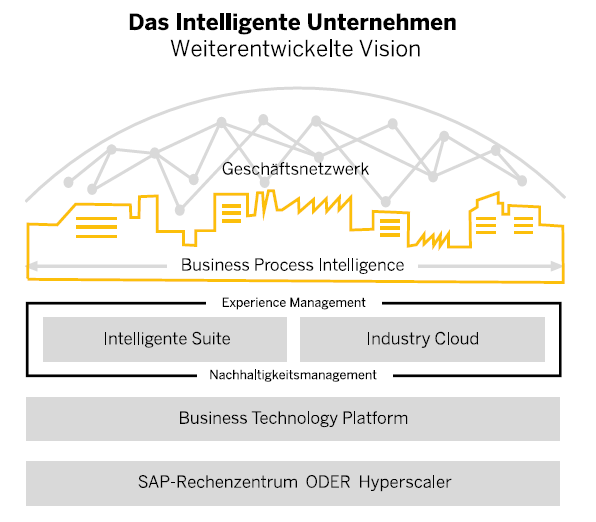
\includegraphics[scale=1]{Bilder/SAPIntelligentesUnternehmen.png}
    \caption[Das Intelligente Unternehmen]{Das Intelligente Unternehmen (\cite[][S. 53]{sap2020-report})}
\end{figure}

Die SAP verfolgt derzeit die Vision ihre Kunden zu einem intelligenten Unternehmen zu entwickeln, in denen die Prinzipien der Innovation, Integration, Agilität und Geschwindigkeit an vorderster Stelle stehen. Außerdem alle Elemente eines Unternehmens verbunden werden und ineinandergreifen. Die Komponenten eines solchen intelligenten Unternehmens sind nach Vorstellungen der SAP ein Geschäftsnetzwerk, das die unternehmensübegreifenden Prozesse miteinander verknüpft, eine Business Process Intelligence, die die Geschäftsprozesse analysiert und optimiert, das Experience Management, das die Daten der Anwender, Kunden und Mitarbeiter analysiert, eine Business Technology Platform, die das Fundament für die Integration und Erweiterung von Anwendungen liefert und dem Kunden Möglichkeiten für künstliche Intelligenz, maschinelles Lernen und Prozessautomatisierung bietet, und einem SAP-Rechenzentrum oder einem Hyperscaler, also einem Infrastrucute-as-a-Service Anbieter wie Amazons AWS oder Microsoft Azure.\footcite[Vgl.][S. 53 f.]{sap2020-report}. Dadurch soll das Ziel erreicht werden, langrfritistig die Abläufe der weltweiten Wirtschaft zu verbessern.


\subsubsection{SAP-ERP}
SAP ERP, oder auch SAP ECC (für SAP ERP Central Component), ist die Weiterentwicklung der dritten Generation des SAP ERP-Systems, \glqq{}SAP R/3\grqq{}, das im Jahr 1992 die zweite Produktgeneration \glqq{}SAP R/2\grqq{} ablöste und im Jahr 2003 in \glqq{}SAP ERP\grqq{} umbenannt wurde.\footcite[Vgl.]{sap-unterschiede} Der Name setzt sich dabei aus dem \glqq{}R\grqq{} für den Begriff \glqq{}Realtime\grqq{}, also Echtzeit, für die Echtzeitdatenverarbeitung und der \glqq{}3\grqq{} zum einen für die dritte Generation, aber auch für die dreischichtigen Architektur, die dem System zugrunde liegt, bestehend aus Datenbank, Anwendungsserver und Client. Die dritte SAP-Generation verfügt dabei über eine zentrale Datenbank, in der alle Daten aus den einzelnen Modulen und den verteilten Anwendungen gesichert werden. SAP ERP bzw. SAP ECC stellt die Zentrale Komponente der \glqq{}SAP Business Suite\grqq{}, in der noch andere Produkte von SAP erhältlich sind, die auf andere Anwendungsbereiche als ERP abzielen, zum Beispiel dem CRM (Customer Relationship Management) oder dem SCM (Supply Chain Management). Durch die unterschiedlich ausgerichteten Systeme können die Kunden sich ihr System frei zusammenstellen und dieses spezifisch an ihr Geschäftsmodell anpassen. Dadurch wird eine noch tiefer gehende Integration von Geschäftsprozessen ermöglicht, da alle diese Systeme mit der selben, zentrale Datenbanken arbeiten.\\ SAP ERP besteht aus unterschiedlichen Modulen, die ebenfalls frei durch die Kunden zusammengestellt werden können.

\begin{figure}[h]
    \centering
    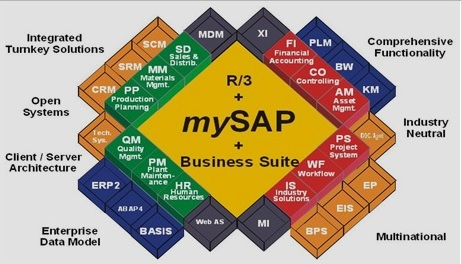
\includegraphics[scale=1]{Bilder/sap-module.jpg}
    \caption[Die Module von SAP-ERP]{Die für SAP-ERP erhätlichen Module (\cite[][]{sap-module})}
    \label{fig:sapmodule}
\end{figure}

In der Abbildung \ref{fig:sapmodule} sind die derzeit für SAP-ERP erhältlichen Module und dazugehörigen Anwendungen bzw. Systeme abgebildet. Die wichtigsten Module und gleichzeitig den Kern des Systems stellen dabei die Module FI, CO, MM, SD, PP und HCM dar, die zum Teil auch standardmäßig in jeder SAP-Installation vorinstalliert sind.\footcite[Vgl.][S. 8]{sap-für-wp} Das Modul FI 
Die aktuellste SAP-ERP Version ist das Enhancementpackage 8 für SAP ERP 6.0 und ist am 04. April 2019 erschienen.

\subsubsection{S/4HANA} 

\subsubsection{SAP HANA}
SAP HANA ist die Datenbanktechnologie, die eigens durch die SAP entwickelt wurde.


\subsection{Transformation}
\subsubsection{Definition}
Unter einer Transformation versteht man im allgemeinen einen grundlegenden Wandel, der durch bestimmte Faktoren, wie z.B. einer sprunghafte wirtschaftlichen, oder technologischen Entwicklung hervorgerufen wird. Die Transformation hält dabei idR. über einen längeren Zeitraum an und ist erst beendet, sobald sich die neu geschaffenen Strukturen etabliert und gefestigt haben.\footcite[Vgl.][]{difu}\\ Im betriebswirtschaftlichen Kontext versteht man unter einer Transformation (oder auch Business Transformation) die gezielte Umgestaltung eines Unternehmens und seiner Geschäftsprozesse, um auf veränderte Bedingungen am Markt einzugehen und sich ihnen anzupassen. Dabei ist das Ziel durch effizientere und vereinfachte Geschäftsprozesse einen Mehrwert in Form von niedrigeren Kosten bei gleichbleibender, oder bestenfalls verbesserter Qualität zu erreichen und dabei zusätzlich die Kundenzufriedenheit zu steigern.\footcite[Vgl.][]{leanix}

\subsubsection{Die vier R der Transformation}
In den 1990er-Jahren wurde durch Gouillart und Kelly das Modell der \glqq{}Vier R der Transformation\grqq{} \footcite[Vgl.][]{4r-modell} entwickelt, was eine mögliche Form der Business Transformation darstellen soll. Aus diesem Modell hat die Beratungsgesellschaft Gemini Consulting (später in der Capgemini SE aufgegangen)\footcite[Vgl.][]{gemini-died} ein Produkt entwickelt, indem die vier R für vier verschiedene Transformationsdimensionen stehen:\\
\begin{figure}[h]
    \centering
    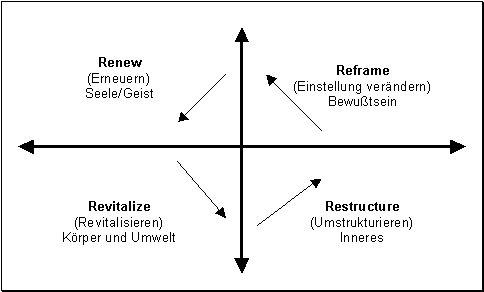
\includegraphics[scale=0.5]{Bilder/businesstransformationManagementportal.png}
    \caption[Die vier R der Transformation]{Die vier R der Transformation (\cite[][]{4r-modell})}
\end{figure}
\begin{itemize}
    \item[] \emph{Reframing (dt. Einstellungsveränderung)} soll in einem Unternehmen dazu beitragen die Sichtweise auf sich selbst zu überdenken um sich dadurch von alten Denkmustern zu befreien. Um diese Einstellungsveränderung anzustoßen ist es wichtig, dass die Mitarbeiter motiviert werden und davon überzeugt sind durch die eingesetze Energie einen Mehrwert zu generieren. Im nächsten Schritt muss anschließend eine Vision definiert werden, die sich erheblich von der präsenten Realität absetzt um im Anschluss daraus Ziele und Messgrößen zu entwickeln. 
    \item[] \emph{Restructuring (dt. Restrukturierung)} 
    \item[] \emph{Revitalising (dt. Wiederbelebung)}
    \item[] \emph{Renewing (dt. Erneuerung)}
\end{itemize}

\subsubsection{Digitale Transformation}
-- Digitale Transformation
\subsubsection{Besonderheiten der S/4HANA Transformation}


%Grundlagen
\section{Unternehmerischer Kontext}
\subsection{Die adesso orange AG}
\subsubsection{Vorstellung des Unternehmens}
Die adesso orange AG ist ein IT-Beratungsunternehmen, das sich vorallem auf die SAP-Beratung spezialisert hat. Sie ist ein Tochterunternehmen der Dortmunder adesso SE, das im Jahr 2021 aus einer Fusion der adesso SE mit der in Hameln ansässigen Quanto AG hervorging. Die adesso SE ist eines der größten IT-Dienstleistungs- und Beratungsunternehmen Deutschlands und hat ca. 5600 Mitarbeiter an 44 Standorten in ganz Deutschland und Europa. \footcite[Vgl.][]{adesso-main} \\Die adesso SE wurde im Jahr 1997 als \glqq{}adesso Beratungsgesellschaft für Software-Prozeß-Management mbH\grqq{} gegründet und hatte Ende der 1990er Jahre erste größere Projekte im Versicherungssektor. Im Jahr 2000 wurde die Gesellschaft mit beschränkter Haftung schließlich zu einer Aktiengesellschaft umgewandelt, zu diesem Zeitpunkt hatte sie bereits 100 Mitarbeiter. Ende der 2000er-Jahre hatte die adesso bereits über 500 Mitarbeiter und erschloss zunehmend die internationalen Märkte in ganz Europa. Im Jahr 2012 erwirtschaftete die adesso AG mit ca. 1000 Mitarbeitern über 100 Mio. Euro Umsatz und vergrößerte sich in den nachfolgenden Jahren durch das Gründen von Tochtergesellschaften stetig. Im Jahr 2019 wurde die adesso AG in eine europäische Aktiengesellschaft \glqq{}Societas Europaea\grqq{} (SE) umgewandelt und war mit über 4000 Mitarbeitern, laut \glqq{}Lünendonk-Liste 2020\grqq{} das größte mittelständische IT-Beratungsunternehmen in Deutschland.\footcite[Vgl.][]{adesso-historie} Im Geschäftsjahr 2020 erreichte die adesso SE eine Umsatzsteigerung von 16 Prozent, im Vergleich zum Vorjahr, auf 523,375 Mio. Euro, wovon ca. 413 Mio. Euro in Deutschland und 110 Mio. Euro im Ausland erwirtschaftet wurden. Von den 523 Mio. Euro waren 60,406 Mio. Euro als Gewinn (EBITDA) zu verzeichnen, was eine Steigerung von 26 Prozent gegenüber dem Vorjahr entspricht. Nach dem Abzug der Abgaben verblieb für das Jahr 2020 ein Konzernergebnis von ca. 21 Mio. Euro.\footcite[Vgl.][S. 4]{adesso2020-report} Besonders sind dabei die Auswirkung der von Anfang 2020 bis dato anhaltenen Covid-19-Pandemie hevorzuheben, die zeitweise zu unterjährigen Wachstumseinbrüchen von bis zu 9,8 Prozent führten. Dies resultierte aus der neuaufgetretenen, allgemeinen Unsicherheit, die unter anderem dazu führte, das adesso-Kunden Projekte stoppten oder verschoben. Das führte dazu, dass Gesellschaften der adesso SE, wie auch viele andere Unternehmen, im Zeitraum von April bis Juli 2020, teilweise Kurzarbeit anmelden mussten und Maßnahmen zur Liquiditätssicherung, wie zum Beispiel der Vereinbarung von Steuerstundungen, veranlassten. Da es sich bei vielen Kunden von adesso um Versicherungen oder Banken handelt, die dem öffentlichen Sektor enstammen, waren die Auswirkungen der Pandemie nicht allzu prikär, was zu einer Erholung im zweiten Halbjahr führte.\footcite[Vgl.][S. 30f]{adesso2020-report} Im zweiten Halbjahr 2020 wurde auch der Mehrheitserwerb an der Quanto AG in Höhe von 71,4 Prozent durchgeführt, der zu der Fusion und später, im Jahr 2021, zu der Neugründung der adesso orange AG führte.\footcite[Vgl.][S. 15]{adesso2020-report} 
\\Mit der adesso orange AG hat die adesso SE den auf SAP spezialiserten Teil ihres Unternehmens, zusammen mit der ehemaligen Quanto AG, in einem seperaten Unternehmen gebündelt, das sich vorallem auf die SAP-Beratung von Banken, Energieversorgern und Versicherungen spezialisiert hat.\footcite[Vgl.][]{ao-main} Derzeit beschäftigt die adesso orange AG ca. 300 Mitarbeiter an den Standorten der adesso SE. Der Hauptsitz befindet sich weiterhin, wie bereits bei der Quanto AG, in Hameln.\footcite[Vgl.][]{ao-karriere}
Die bis 2021 bestehende Quanto AG ging im Jahr 2016 aus dem Zusammenschluss der Firmen \glqq{}Aequitas\grqq{} und \glqq{}Quanto\grqq{} hervor, um gemeinsam größere Kunden zu gewinnen.\footcite[Vgl.][]{ww-quanto} Die Quanto AG hielt bereits Standorte in Hamburg, Kiel, Flensburg, Stuttgart, Heidelberg, Berlin sowie im ungarischen Budapest und Györ und hatte bereits im Jahr 2016 ca. 140 Mitarbeiter. Neben den Bereichen der SAP konzentrierte sich die Quanto AG auch auf das \glqq{}Internet der Dinge\grqq{} und Blockchain-Technologien.\footcite[Vgl.][]{ww-quanto}

\subsubsection{Geschäftsmodell}
Bei der adesso orange AG handelt es sich um ein Dienstleistungsunternehmen, das sich auf die SAP-Beratung im öffentlichen Sektor spezialisiert hat. Als Beratungsunternehmen verfolgt die adesso orange AG das Ziel, die Unternehmensstrategie ihrer Kunden in eine angepasste SAP-Architektur zu übersetzen. Die soll geschehen, indem die Unternehmensprozesse in ihrer Gänze betrachtet und analysiert werden und diese anschließend, mit dem mitgebrachten Fachwissen, in eine SAP-Lösung überführt werden.\footcite[Vgl.][]{ao-main} Als Beratungsunternehmen versucht die adesso orange AG als externe Organisation ihren Klienten, durch eine personalisierte Aufarbeitung einer betriebswirtschaftlichen Problemstellung, zu einer Lösung dieses Problems zu verhelfen. Diese Unterstützung kann entweder technischer oder organisatorischer Natur sein und wird an die Erwartungshaltung des Klienten angepasst, sowie an das durch die Berater angebotene Leistungsspektrum.\footcite[Vgl.][]{gabler-beratung}
\begin{figure}[h!]
    \centering
    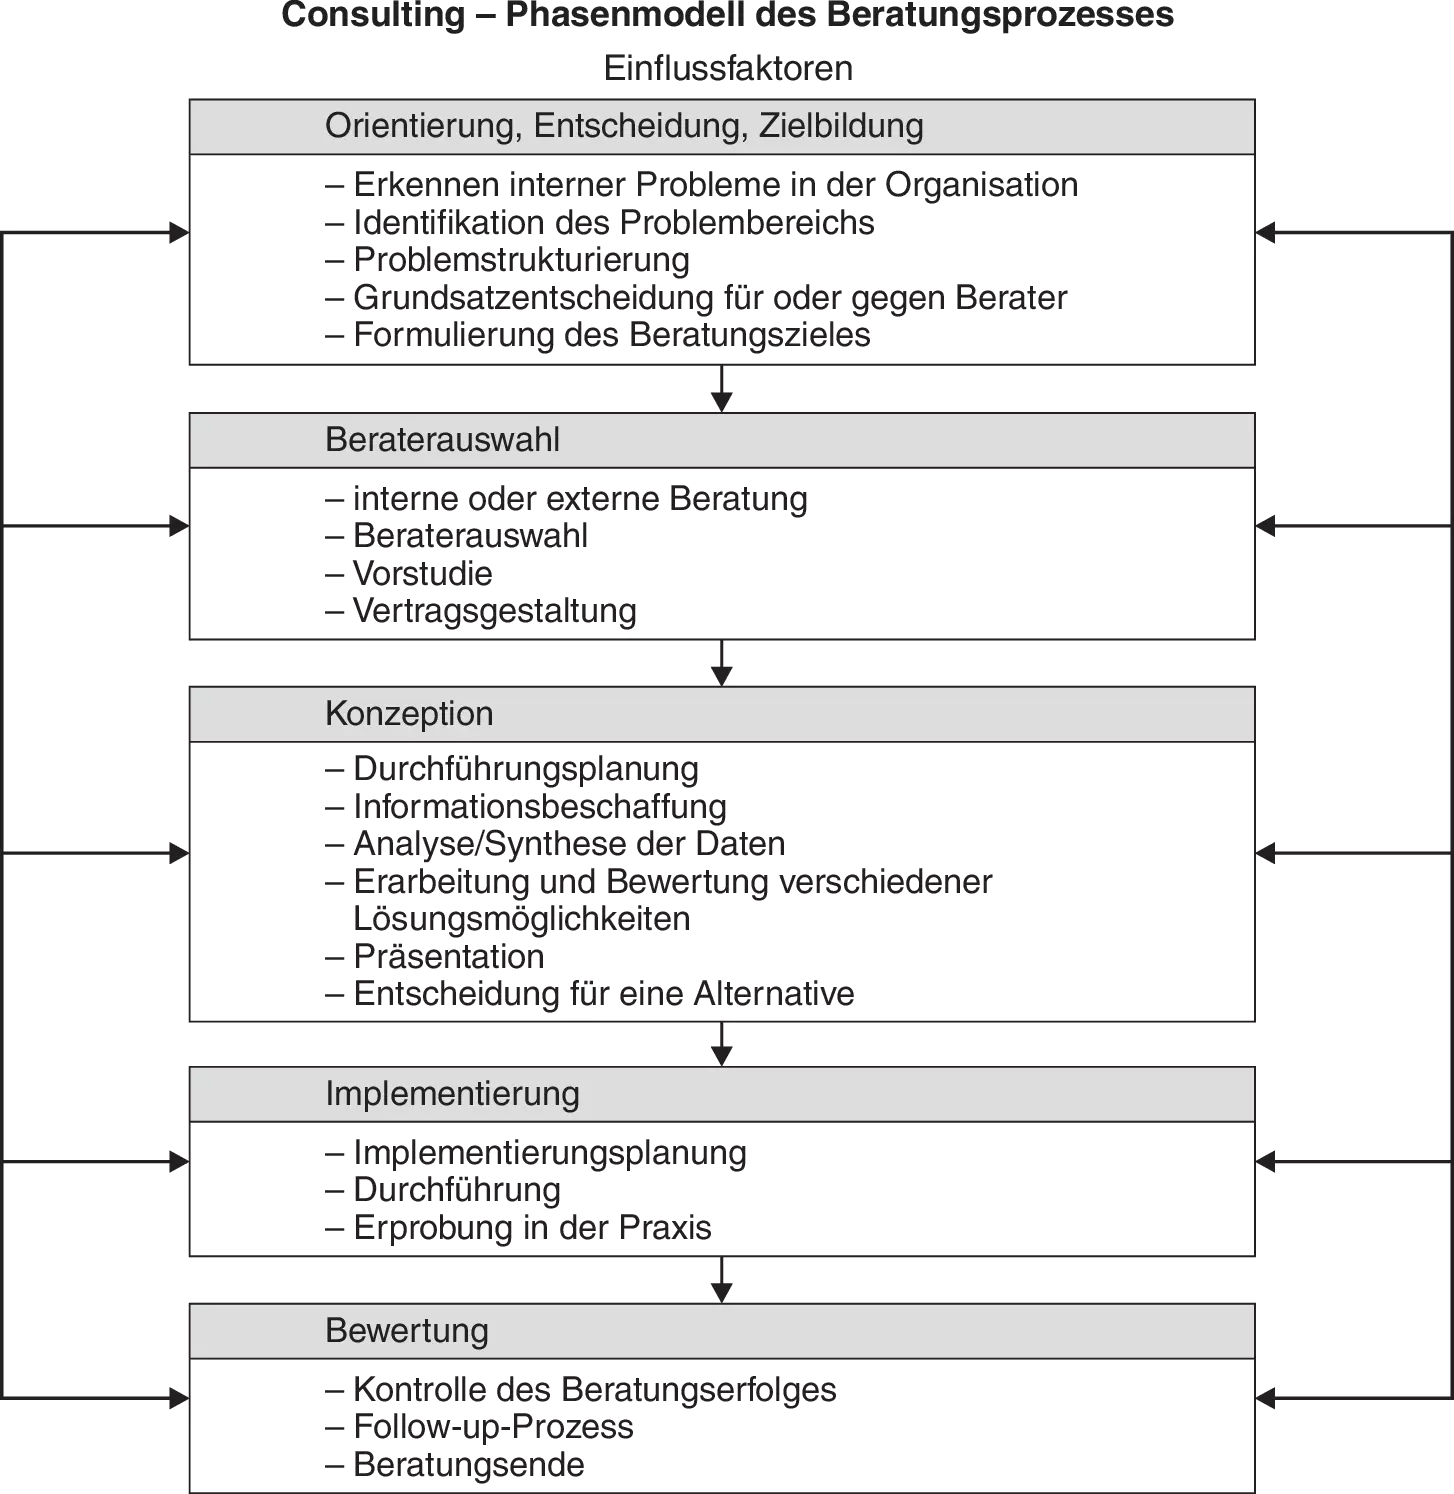
\includegraphics[scale=0.4]{./Bilder/Beratungsprozess.png}
    \caption[Phasenmodell eines Beratungsprozess]{Phasenmodell eines Beratungsprozess (Quelle: \cite[][]{gabler-beratung})}
\end{figure}
\\In der Praxis findet die Beratung in der Regel innerhalb von Projekten beim Kunden statt, die damit beginnen, dass der Kunde entweder auf das Beratungsunternehmen zukommt, oder eine Ausschreibung anfertigt, auf die sich das Beratungsunternehmen bewirbt. Danach erfolgt die Angebotserstellung durch das Beratungsunternehmen, in dem der Umfang des Projekts und die Leistungen der Berater festgehalten sind, sowie das Projektbudget. Die Abrechnung eines Projektes erfolgt entweder pauschal über einen Festpreis, oder über einen Stundensatz anhand der geleisteten Arbeitszeit. Sobald der Angebotszuschlag erhalten wurde, beginnt das Projekt mit der Konzeptionsphase, in der Informationen beschafft, Daten analysiert und verschiedene Lösungsmöglichkeiten in einem Fachkonzept erarbeitet werden. Sobald sich der Kunde für eine der Lösungen entschieden hat, beginnt mit der Implementierung die nächste Projektphase. In dieser findet die Durchführung der Lösung statt, sowie im Anschluss Tests und Fehlerbehebungen. Nach dem Abschluss der Implementierungsphase erfolgt die Abnahme, bzw. die Bewertung durch den Kunden, der auch eventuelle Nacharbeiten festsetzt oder nachfolgende Projekte in Aussicht stellt.\footcite[Vgl.][]{gabler-beratung}
\\Durch das nahende Supportende von SAP ERP (R/3) im Jahr xxxx (siehe Kapitel \ref{kap:R3}) stehen zur Zeit viele Unternehmen unter Zugzwang auf die neuste Generation S/4HANA zu aktualisieren. Dadurch ergeben sich für die Beratungsbranche viele Möglichkeiten Aufträge in Form von S/4HANA-Transformationsprojekten zu aquirieren. Auf der anderen Seite bietet der Druck auf die Unternehmen aber auch Chancen im selben Zug einschneidene Änderungen an den in SAP abgebildeten Geschäftsprozessen vorzunehemen, indem sich von Eigenentwicklungen und ineffizienten Prozessen getrennt wird und sie durch Prozesse des gängigen Industriestandard ersetzt.

\subsection{Vorgehensmodell S/4HANA Transformation}
\subsubsection{Aufbau}
Die adesso orange AG hat für die Durchführung von SAP S/4HANA Transformationen, mit Hilfe der im Unternehmen ansässigen Expertise, ein eigenes Vorgehensmodell entwickelt, dass auf verschiedenen Projektphasen und Bausteinen basiert um eine Transformation von IT-Systemen und -Landschaften durchzuführen, vorallem aber auch um S/4HANA-Transformationen (siehe Kapitel \ref{kap:s4hanatrans}) zu vollziehen. Dieses Vorgehensmodell wird unter dem Produktnamen \glqq{}adesso active transformation\grqq{} vermarktet und kam bereits in einigen größeren S/4HANA-Transformations-Projekten zum Einsatz. Ziel dieses Vorgehensmodell ist die Transformation strukturiert zu durchlaufen und dabei alle Aspekte von der Planung bis zur Umsetzung zu berücksichtigen. Wie bereits erwähnt, basiert das Modell auf verschiedenen Phasen, die widerrum unterschiedliche Bausteine enthalten, die einzelne Leistungen abbilden, die z.B. in Form von Workshops (Arbeitsgruppen) oder Konzepten. Mit Hilfe dieser Bausteine, kann individuell, je nach Anforderungen der Kunden, ein Projekt effektiv durchgeplant werden. Des Weiteren werden während einer Transformation verschiedene \glqq{}Streams\grqq{} (Flüsse) betrachtet, die parallel zu einander laufen und sich durch das gesamte Projekt ziehen. Diese Streams bündeln die einzelnen Aktivitäten, z.B. technischer, organisatorischer, oder betriebswirtschaftlicher Natur sind. Das erklärte Hauptziel der \glqq{}adesso active transformation\grqq{} ist zum einen die Ermittlung eines optimalen Transformationspfades des betrachteten Systems, die Erstellung eines Umsetzungskonzeptes für die Transformations, sowie die letzendliche Umsetzung der Transformation in einer strukturierten Arbeitsweise.\footcite[Vgl.][]{aat-vorgehensmodell}

\subsubsection{Phasen}
Nachfolgend werden die einzelnen Projektphasen des Vorgehensmodell beschrieben, und ihre jeweiligen Bausteine zusammengefasst. In Abbildung \ref{fig:AAT} sind die einzelnen Phasen in einer Übersicht abgebildet.
\begin{figure}[!h]
    \centering
    \includegraphics[scale=0.65]{./Bilder/AAT-Überblick.png}
    \caption[Phasen des Vorgehensmodell]{Phasen der adesso active transformation (Quelle: \cite[][]{aat-phasen})}
    \label{fig:AAT}
\end{figure}
\\Das Vorgehensmodell beginnt mit der \underline{\glqq{}Enterprise Discover\grqq{}-Phase}, die das Ziel hat das Kundenunternehmen für eine Transformation vorzubereiten und die strategischen Möglichkeiten der Vorgehensweise offen zulegen. In dieser Phase wird, wie der Name der Phase bereits andeutet, das Unternehmen, bzw. die Unternehmenslandschaft und Unternehmensarchitektur erkundet, um eine initiale Übersicht über das Unternehmen zu erhalten, mit allen Aspekten, die während einer Transformation berücksichtigt werden müssen. Des Weiteren finden diverse Beratungsgespräche zusammen mit den Kunden statt, in denen dem Kunden mögliche Wertschöpfungspotenziale und Gedankenanstöße für die Durchführung einer Transformations erörtert. Auch findet zu Beginn eine Evaluierung der Projektmethodik statt, in der entschieden wird, ob das Projekt, im Falle eines Angebotszuschlags durch den Kunden, klassisch nach Wasserfallmodell, agil oder als eine hybdride Mischung der beiden Methodiken stattfinden soll. Zum Ende der Enterprise-Discover-Phase findet die Ermittlung des Projektumfangs statt, in der aufgelistet wird, wieviele zu transformierende Geschäftsprozesse es gibt, welche Prozesse neu abgebildet werden sollen, welche Werkzeuge im Projekt eingesetzt werden sollen und ob es übergreifende Themen gibt, die über das gesamte Projekt verteilt stattfinden müssen (z.B. Testmanagement). Dies ist zugleich auch das Ergebnisobjekt der ersten Phase und die Grundlage für die zweite Phase.\footcite[Vgl.][]{aat-enterprisediscover}\\
\vspace{1em}
\\Die zweite Phase in der adesso active transformation ist die \underline{\glqq{}Prepare\grqq{}-Phase}, die zum Ziel hat die in der ersten Phase ermittelten Geschäftsprozesse ganzheitlich aufzunehmen und die Anforderungen aus der IT im Bezug auf die Transformation zu erfassen. Im Vorfeld findet jedoch zuerst eine UX-Journey (Vorstellung der Benutzeroberfläche) statt, in der ein neu aufgesetztes S/4HANA-System im Greenfield-Zustand dem Kunden präsentiert wird und dabei auf die Neuerungen eingegangen wird. Im Anschluss folgen weitere Präsentationen auf Modulebenen mit den jeweiligen Fachbereichen des Unternehmen, in denen weitere Anforderungen an die Transformation ermittelt werden. Die Ergebnisse dieser Vorstellungen wird im Anschluss dokumentiert und zusammengefasst und dienen der Definition des Tranformationspfads, also welcher Ansatz zur S/4HANA-Transformation verfolgt werden soll. Ebenfalls werden in der Prepare-Phase die momentanen Reporing- und Planungsprozesse aufgenommen und die neuen Business Intelligence Funktionen von SAP S/4HANA präsentiert. Zum Ende dieser Phase werden die einzelnen Ergebnissobjekte zu einem ersten Konzept konsolidiert, das als Basis der dritten Phase dient. Am Ende der Prepare-Phase steht ein \glqq{}Quality Gate\grqq{}, also eine Abnahme durch den Kunden, in der Kunde überprüft, ob die an das Projekt gestellten Anforderungen erfüllt werden.\footcite[Vgl.][]{aat-prepare}\\
\vspace{1em}
\\Die dritte Phase in der adesso active transformation ist die \underline{\glqq{}Explore\grqq{}-Phase}, die zum Ziel hat, die Ergebnisse der zweiten Phase in ein Feinkonzept zu überführen. Ebenfalls erfolgt in dieser Phase die Vorbereitung der technischen Systeme auf die Umsetzung in der nächsten Phase. Diese Vorbereitung besteht zu einen aus dem Aufsetzen von Entwicklungs-, Test- und Produktivsystemen aber auch aus der Bereitstellung der Systenmzugänge für die Projektmitarbeiter in den neuen, sowie in den alten Systemen. Ein weitererer Punkt in der Explore-Phase ist das Thema Authetifizierung und Sicherheit, indem es zum einen um die Sicherheit des System, also um das erstellen eines Berechtigungskonzept geht, in dem entweder die Übernahme von bestehenden Strukturen beschlossen wird, oder ein kompletter Neuaufbau der Rollen und Berechtigungen beschrieben ist. Zum anderen geht es aber auch um die Datensicherheit, in dem regelmäßige Datensicherungen durchgeführt werden und die Anforderungen der Europäischen Datenschutz Grundverordnung (EU-DSGVO) zum Speichern von personenbezogenen Daten erfüllt werden müssen. Das Ergebnisobjekt der Prepare-Phase ist das Feinkonzept, was die Basis für die Umsetzung in der nächsten Phase darstellt.\footcite[Vgl.][]{aat-explore}\\
\vspace{1em}
\\In der vierten Phase, der \underline{\glqq{}Realize\grqq{}-Phase}, geht es schließlich um die Umsetzung des Feinkonzepts. Dies geschieht, indem das neue System konfiguriert und an die Bedürfnisse des Kunden angepasst wird. Dazu werden, je nach Konzept, die Geschäftsprozesse des Unternehmen neu im System abgebildet oder aus dem Altsystem übernommen. Ebenfalls werden die nachwievor benötigten Eigenentwicklungen entweder übernommen oder im S/4HANA neu aufgebaut. Da je nach Projekt auch historische Daten aus dem Altsystem übernommen werden, müssen auch die in das neue System migriert werden. Aufgrund der Änderungen in der Datenstruktur in S/4HANA müssen hierzu Umschlüsselungen der Datenbanktabellen stattfinden, damit die Daten übernommen werden können. Ein weiteres wichtiges Thema ist das anschließende Testen des Systems und der Prozesse. Dies muss strukturiert erfolgen, damit alle Geschäftsprozesse, in allen Variationen, vollständig getestet werden, um Fehler zu erkennen und diese zu beheben. Zum Ende der Realize-Phase erfolgt die Abnahme durch den Kunden, in der überprüft wird, ob alle Prozesse und Systeme wie gewünscht funktionieren, alle Anforderungen erfüllt wurden und ob das S/4HANA-System in den produktiven Betrieb gehen kann.\footcite[Vgl.][]{aat-realize}\\
\vspace{1em}
\\Der \underline{\glqq{}Go-Live\grqq{}} und die anschließenden Nacharbeiten stellen die fünfte Projektphase in der adesso active transformation dar. Hierbei erfolgt nach der erfolgreichen Abnahme des Systems durch den Kunden, der Go-Live, also die Produktivsetzung des Systems. Da, aufgrund der intensiven Nutzung nach Go-Live, häufig auch dann noch Fehler auftreten, werden diese durch das Projektteam nach Go-Live behoben. Auch kann es vorkommen, dass in diesem Zeitraum noch nachgelagerte Aktivitäten stattfinden, die von vorhinein niedrig priorisiert wurden. Ebenfalls werden in diesem Zeitraum häufig die Dokumentationen und die Anwenderhandbücher noch finalisiert und dem Kunden übergeben. Nach der Go-Live-Phase kann durch den Kunden noch ein individueller Wartungsvertrag geschlossen werden, in dem beschlossen ist, das auch nach Ende des Projekts Fehlerbehebungen stattfinden.\footcite[Vgl.][]{aat-golive}


\subsubsection{Werkzeuge}
Das adesso active Transformation Vorgehensmodell sieht neben den verschiedenen Projektphasen auch phasenübergreifende Werkzeug vor, die zum Einsatz kommen und die Projektmitarbeiter unterstützen soll. \\Dies ist zum einen die Webanwendung \underline{\glqq{}Jira\grqq{}} vom Softwarehersteller Atlassian, die sich für die systematische Projektsteuerung und das Nachverfolgen von Aufgaben eignet, aber auch Funktionen für das Melden von Fehlern (bug reporting) vorsieht. In Jira lassen sich verschiedene Teilprojekte in Form von Komponenten aufbauen und Meilensteine in Form von Releases abbilden. Für das Vorgehensmodell ist ein Jira-Vorlage vorgesehen, mit dem ein Projekt in Jira angelegt werden kann, indem bereits die Grundkonfiguration vorgenommen wurde.\\
Ebenfalls ist in der adesso active Transformation eine Excel-Spreadsheet-Vorlage zur Durchführung des Projektcontrollings vorgesehen. Dieses Spreadsheet dient zur Unterstützung der Projektleitung, indem diese das Projektbudget verwalten und den Einsatz der Projektmitarbeiter planen kann. Sobald das Spreadsheet an das entsprechende Projekt angepasst und konfiguriert ist, können die vorgesehenen Projekttage der Projektmitarbeiter erfasst und über den gesamten Projektzeitraum vorrausgeplant werden.  
Das Tool ermöglicht zudem den Import von erfassten Arbeitszeiten über eine Schnittstelle zu dem von adesso orange eingesetzten Zeiterfassungstool \glqq{}ZEP\grqq{}. Somit kann die Projektleitung zu jedem Zeitpunkt einen Soll-Ist-Vergleich vornehmen und ggf. das Budget umverteilen oder zusätzliche Projekttage beantragen.

\subsubsection{Business Transformation Tracker}
Ein weiteres wichtiges Tool im Vorgehensmodell ist der \underline{\glqq{}Business Transformation Tracker\grqq{}} (BTT) der zum momentanen Zeitpunkt durch ein Excel-Spreadsheet implementiert ist. In diesem werden zu Beginn des Projektes, in der Prepare-Phase, die Geschäftsprozesse, die es zu transformieren gilt, ganzheitlich erfasst. Dazu werden die Prozesse in Subprozesse und Prozessschritte aufgespalten und Schritt für Schritt in dem Business Transformation Tracker eingetragen. Im BTT sind je Projektphase verschiedene Kriterien hinterlegt, durch die die Vollständigkeit der Transformation je Prozessschritt ermittelt wird. Diese Kriterien können entweder Eigenschaften oder Aufgaben sein, deren Erfüllung im BTT dokumentiert wird. In der Regel gibt es pro Teilprojekt im Transformationsprojekt einen Business Transformation Tracker in Form eines Excel-Spreadsheets.\\
Da diese Umsetzung schnell Unübersichtlich wird und der Funktionsumfang auch nur begrenzt ist, besteht bei adesso orange der Wunsch, die momentan implementierte Excel-Lösung in ein eigenes System zu überführen. Die Konzeption dieser Überführung in ein eigentständiges Systems wird nun in den folgenden Kapiteln behandelt.

%Methodik
\section{Methodik}
\subsection{Erhebung des Ist-Zustandes}
Der Softwareentwicklungsprozess wurde im Studiengang Wirtschaftsinformatik der Hochschule Hannover ausgiebig behandelt und setzt sich aus 





\subsection{Requirements Engineering}
\subsubsection{Vorgehensmodell nach Balzert}
Umfrage der MA
\subsection{Vorgehen}
%Anfang nochmal ändern 
Dazu wird zunächst auf die einschlägigen Begrifflichkeiten eingegangen um sich dann dem Themenkomplex der S/4HANA-Transformation zu nähern und ihre Eigentschaften und Besonderheiten zu erklären. Im Anschluss wird zuerst das Unternehmen, in dessen Kontext sich diese Arbeit abspielt, vorgestellt, um dann genauer auf das Geschäftsmodell und das Vorgehensmodell zur S/4HANA Transformation einzugehen. \\
Danach wird der aktuelle Ist-Zustand des Tools, bzw. die Form, die momentan verwendet wird, vorgestellt und genauer darauf eingegangen, warum diese Form durch eine Neuentwicklung ersetzt werden sollte. Schließlich wird die Konzeption des Programms stattfinden. Dazu werden im ersten Schritt die Anforderungen analysiert, indem Interviews mit unterschiedlichen Key-Usern und Stakeholdern geführt werden, um daraus verschiedene Anwendungsfälle und -beispiele heraus zu filtern. In der Anforderungsanalyse werden sich ebenfalls Geschäftsprozessmodelldiagramme, erste Klassendiagramme und Sequenzdiagramme wiederfinden, um die Anforderungen an die Entwicklung zu visualisieren. Im nächsten Schritt werden die erarbeiteten Anforderungen ausgeprägt


%Ist-Zustand
\section{Erhebung des Ist-Zustand}

\subsection{Was bietet das Tool bereits heute}
Zum jetzigen Zeitpunkt exisitiert der Business-Transformation-Tracker bereits in Form eines Excel-Spreadsheets. Dieses wird bereits in einigen Transformationsprojekten des betrachteten Unternehmens verwendet und unterstützt dadurch schon heute die Mitarbeiter in den Projekten. \\Das Tool dient dazu in einem S/4HANA Transformationsprojekt 
\subsection{Welche Verbesserungspotenziale gibt es}

\subsection{Warum verbessern?}

\subsection{Geplante Erweiterungen des Funktionsumfangs}

\subsection{Interviews mit Stakeholdern}

%Anforderungsermittlung
\section{Ermittlung der Anforderungen}
\subsection{Ermittlung der Stakeholder}
Bevor mit der Ermittlung der Anforderungen begonnen wird, müssen zuerst die Stakeholder identifiziert werden, die ein allgemeines Interesse an der zu entwicklenden Software, bzw. dem Tool haben. Dabei handelt es sich um Personen, die entweder von dem fertigen Produkt profitieren, oder die später das Produkt zu ihrer täglichen Arbeit einsetzen und daher ein Interesse am Funktionsumfang und der Benutzerfreundlichkeit haben. 

\subsubsection{Analyse der Stakeholder}
Im Falle des Business-Transformation-Trackers wurde folgende Stakeholder ermittelt:
\begin{itemize}
    \item[] \emph{Oberes Management:} Das obere Management des auftraggebenen Unternehmens ist der Auftraggeber für das Entwicklungsprojekt und hat daher besonderes Interesse in der erfolgreichen Fertigstellung des Projekts und der produktivsetzung der Software um somit Wertschöpfung zu generieren. Dazu kommt, dass das Ziel der Software die Unterstüzung der Mitarbeiter in den Projekten ist und sich durch den Einsatz eine Effizienzsteigerung und Qualitätsverbesserung erhofft wird. Dadurch besteht die Möglichkeit der Reputationssteigerung gegenüber potentiellen Kunden und somit einer gesteigerten Nachfrage im Vertrieb, was ebenfalls im besonderen Interesse des Managements liegt. In Persona tritt das obere Management im Entwicklungsprojekt als Bereichsleiter \glqq{}SAP Consulting and Development\grqq{} in Erscheinung.
    \item[] \emph{Mittleres Management:} Die Mitarbeiter des auftraggebenen Unternehmen im mittleren Management fungieren in der Regel in der Rolle eines Abteilungs- oder Projektleiters und haben daher ein besonderes Interesse an dem Funktionsumfang an der zu entwicklenen Software, da sie durch den Funktionsumfang direkt in den Projekten profitieren können. So profitieren sie beispielsweise von einer übersichtlichen Ansicht des gesamten Projekts und können durch Auswertungen besser das Projekt verwalten. Außerdem besitzen die Mitarbeiter des mittleren Managements ein Interesse darin, dass das Tool durch die Mitarbeiter verwendet wird, damit die darin geführten Daten stets auf dem aktuellen Stand sind. 
    \item[] \emph{Senior Consultants:} Senior Consultants sind erfahrene Mitarbeiter des auftraggebenen Unternehmens und arbeiten in der Regel als Projektleiter in kleineren Projekten oder als Teilprojektleiter in Projekten mit größerem Umfang. Sie haben ein großes Interesse im Funktionsumfang des BTT und sind auch sehr an der Übersichtlichkeit und Benutzerfreundlichkeit der grafischen Oberfläche interessiert, da sie, zusammen mit den Consultants, am intensivsten mit dem Programm arbeiten werden. Dabei stehen die Ziele der Datenkonsistenz und der generellen Verfügbarkeit des BTT im Vordergrund, damit eine reibungslose Arbeit ermöglicht wird.
    \item[] \emph{Consultants:} Die Consultants, bzw. Berater bilden den Kern der Mitarbeiterschaft des auftraggebenen Unternehmens und treten in der Regel als Projektmitarbeiter in Erscheinung. Sie bilden die größte Zielgruppe, da sie am häufigsten mit dem Programm arbeiten werden und dort den Großteil der Datenerfassung durchführen werden. Deshalb ist es vom besonderen Interesse, den Projektmitarbeitern die Arbeit mit dem Produkt möglichst einfach zu machen und besonders auf die Benutzerfreundlichkeit in der Entwicklung zu achten. Dazu kommt, das es wichtig ist, diese Stakeholdergruppe möglichst in die Entwicklung mit einzubeziehen, um Verbesserungsvorschläge und Ideen in die Anforderungen mit aufzunehmen. 
    \item[] \emph{Entwickler:} Die (SAP-)Entwickler des Auftraggebers spielen nur eine untergeordnete Rolle im Kontext des Business Transformation Tracker, da die Befüllung und Auswertung nicht in ihr Aufgabenfeld gehört. Denkbar sind dennoch Szenarien, in denen sie aufgefordert werden einzelne Einträge in dem Programm vorzunehmen, zu denen ihre Expertise benötigt wird. Auch besteht ein großes Interesse an Benutzerfreundlichkeit und Übersichtlichkeit, damit auch bei seltener Nutzung der Umgang mit dem Programm nicht schwer fällt.
    \item[] \emph{Kunden:} Weitere Stakeholder sind die Kunden des Auftraggebers, da diese ebenfalls Berührungspunkte mit dem Programm haben werden, wenn es Teil ihres Transformationsprojekts wird. Sie haben ein besonderes Interesse an der gesteigerten Effizienz und der gesteigerten Qualität ihrer Transformation, da dies für sie eingesparte Ressourcen in Form von weniger Projekttagen, weniger Aufwänden für die Transformation und geringere Wartungskosten im Anschluss durch die gesteigerte Qualität der Prozesse bedeutet. Dazu kommt, dass es dazu kommen kann, dass in größeren Projekten die Mitarbeiter des Kunden ebenfalls in direkten Kontakt mit dem BTT kommen, um bspw. bei der Erfassung der Prozesse zu unterstützen. Dadurch entsteht ein großes Interesse an der Übersichtlichkeit und der Benutzerfreundlichkeit, damit auch bei einmaliger Benutzung das gewünschte Resultat zustande kommt.
\end{itemize}

\subsubsection{Riskobewertung der Stakeholder}
Von den unterschiedlichen Stakeholdern gehen unterschiedliche Risiken im Bezug auf den Erfolg des Produkts aus. So gibt es auf der einen Seite ein unterschiedliches Konfliktpotential, das durch die unterschiedliche Mächtigkeit der Stakeholder, verschiedene Probleme im späteren Einsatz des Tools herbeiführen kann. So wäre es zum Beispiel denkbar, dass ein Consultant die Arbeit mit dem BTT verweigert, wenn seine persönlichen Anforderungen, in Form von Benutzerfreundlichkeit, außer Acht gelassen werden, oder, das ein Mitarbeiter des mittleren Managements, in Form eines Projektleiters, den Einsatz von Anfang an garnicht erst vorsieht, wenn er der Meinung ist, dass das Tool keinen Mehrwert bietet, wenn seine Anforderungen an das Programm, beispielsweise in Form von Verfügbarkeit und Zuverlässigkeit, nur unzulänglich erfüllt werden.
\begin{figure}[ht]
    \centering
    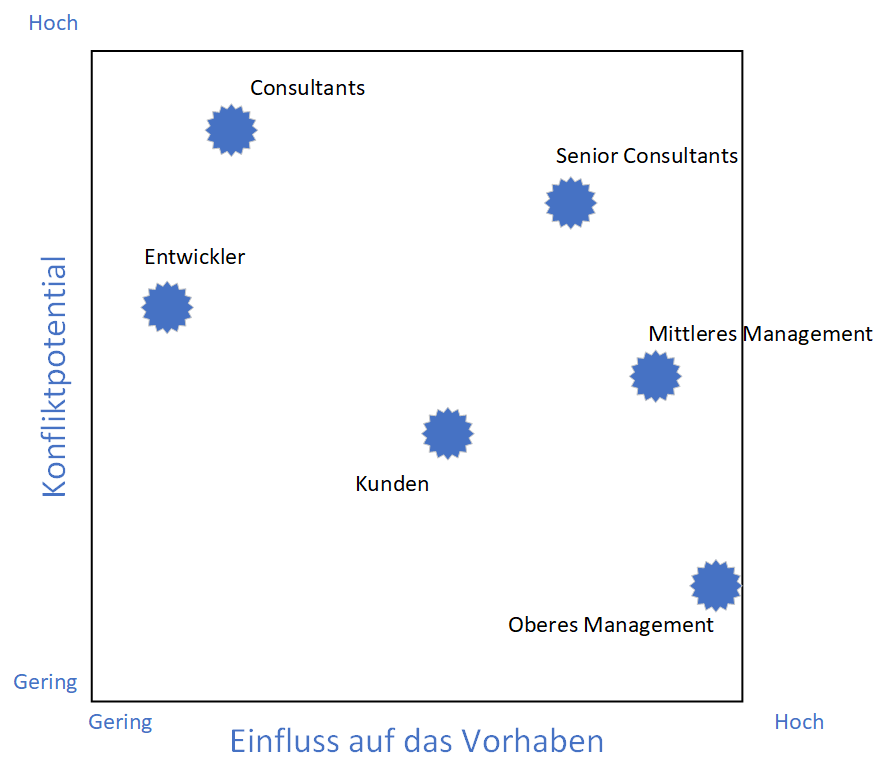
\includegraphics[scale=0.67]{Bilder/stakeholderRisiko.png}
    \caption[]{Subjektive Risikobewertung der genannten Stakeholder}
\end{figure}
Dieses Konfliktpotential lässt sich umgehen, indem die Personengruppen frühzeit in die Anforderungsermittlung mit eingebunden werden und sie dadurch, im Rahmen der Möglichkeiten, selbst bei der Produktentwicklung mitwirken können. Besonders bei Stakeholdern mit großer Macht und hohem Konfliktpotential ist es daher wichtig Maßnahmen zu definieren, wodurch dieses gesenkt werden kann.\footcite[Vgl.][S. 504 f.]{balzert}



\subsection{Erhebung der Anforderungen}
\subsubsection{Informationen durch den Auftraggeber}
Zur Ermittlung der Anforderungen fanden mehrere Gespräche mit dem Auftraggeber statt, in denen zum einen auf den aktuellen Ist-Zustand eingegangen wurde, aber auch Ideen und Umsetzungsvorschläge besprochen wurde. Diese Informationen wurden bereits in dem vorangegangenen Kapitel 5 in der Problemstellung und in der Beschreibung des Ist-Zustandes untergebracht und werden nun genutzt um daraus die Anforderungen an das in Auftrag gegebene Programm zu entwickeln. Während des Entwicklungsprozess besteht ein enger Kontakt zu dem Auftraggeber, wodurch auftretene Rückfragen schnell beantwortet werden können. 

\subsubsection{Befragung im Unternehmen}
Um von möglichst vielen Stakeholdern Anforderungen an eine Neuentwicklung des Business Transformation Trackers zu erhalten, wurde mit den Mitarbeitern des auftraggebenen Unternehmen, die bereits mit der aktuellen Umsetzung des BTT, bzw. seinem Vorgänger, gearbeitet haben, eine Onlinebefragung durchgeführt. Ziel der Befragung war es zum einen das generelle Meinungsbild der Mitarbeiter zu dem BTT zu erfassen und zum anderen mögliche Verbesserungsvorschläge und Ideen der Stakeholder aufzugreifen, um daraus Anfoderungen an einen Neuaufbau des BTT zu entwickeln. Die Umfrage richtet sich dabei an alle internen Stakeholder, das heißt an die Mitarbeiter des oberen und mittleren Mangements, an die Senior Consultants, Consultants und Entwickler. Dadurch soll ein möglichst breites Bild entstehen, dass alle Interessen abdeckt, sodass kein Stakeholder vernachlässigt wird.\\Die Umfrage wurde mit der Online-Plattform \glqq{}Microsoft Teams\grqq{} umgesetzt, das Bestandteil der im Unternehmen eingesetzen Softwaresuite \glqq{}Microsoft 365\grqq{} ist. Die Umfrage wurde anonym durchgeführt, mit der Möglichkeit am Ende freiwillig seine Kontaktdaten anzugeben, um Rückfragen zu den gegebenen Antworten und Vorschlägen zu ermöglichen. Der Fragenkatalog bestand aus drei Abschnitten, zuerst allgemeine Fragen zur Person und zur Position im Unternehmen, als nächstes mit Fragen zur Meinung über den BTT und zum Schluss mit der Möglichkeit Verbesserungsvorschläge und Ideen anzugeben. Um dem Betriebsklima im Unternehmen gerecht zu werden, wurde in der Umfrage auf die förmliche Anrede der Befragten verzichtet.

\subsubsection{Auswertung der Umfrage}

\subsection{Spezifikation der Anforderungen}
Im nun folgenden Unterkapitel werden die im letzten Kapitel, durch Onlinebefragung und in persönlichen Gesprächen, ermittelten Anforderungen spezifiziert, das heißt, systematisch ausgewertet. Es wird aufgrund einer nichtvorhandenen Ausschreibung des Projekts und des geringen Projektumfangs auf ein seperates Lasten- und Pflichtenheft verzichtet und stattdessen die Anforderungen in der hier beginnenden \glqq{}Requirements Specification\grqq{}, zu deutsch \glqq{}Anforderungsspezifikation\grqq{}, niedergeschrieben. Dazu wird sich an der von Helmut Balzert beschriebenen \glqq{}Schablone[n] für Lastenheft, Pflichtenheft und Glossar\grqq{}\footcite[S. 492]{balzert} orientiert. In dieser werden zuerst die Visionen und Ziele des Entwicklungsprojekt verfasst, danach die Rahmenbedingungen denen die Entwicklung unterliegt, im Anschluss der technische Kontext, in dem sich die Entwicklung abspielt und dann erst die funktionalen Anforderungen, die die Kernfunktionalität des Systems beschreiben gefolgt von den nichtfunktionalen Anforderungen, bzw. den Qualitätsanforderungen, in denen die messbare Qualität und das Verhalten des Systems beschrieben wird.\footcite[Vgl.][S. 492 ff.]{balzert}. Die Anforderungen sind natursprachlich verfasst und verfügen über einen einzigartigen Identifikator, um im späteren Verlauf auf sie verweisen zu können. Diese sind so aufgebaut, dass \glqq{} [j]ede Anforderung [..] mit einem Buchstaben [beginnt] [...], gefolgt von einer Zahl, eingschlossen in Schrägstriche. Der Anforderungstyp wird durch einen Buchstaben gekennzeichnet [...]. Am Anfang werden  die Zahlen in Zehnerschritten durchnummeriert, sodass spätere fachlich dazugehörige Anforderungen zwischgefügt werden können.\grqq{} \footcite[S. 493]{balzert}

\subsubsection{Visionen und Ziele}
Die hier aufgezählten Visionen und Ziele sind Ausdruck der mit dem fertigen Produkt zu erreichenden Zukunft. Visionen sind dabei abstrakter und generisch verfasst, Ziele konkretisieren diese dann im Anschluss.\footcite[Vgl.][S. 457]{balzert}
\begin{itemize}
    \item[] \emph{/V10/} Der Auftraggeber soll durch den Business Transformation Tracker eine Qualitätssteigerung und Effizienzverbesserung in seinen Transformationsprojekten erreichen.
    \item[] \emph{/V20/} Die Anwender sollen mit dem Business Transformation Tracker während des gesamten Projektzeitraums die in SAP umgesetzten Prozesse erfassen und nachverfolgen können.
    \item[] \emph{/V30/} In jedem adesso active transformation -Projekt soll der Business Transformation Tracker eingesetzt werden.
    \item[] \emph{/V40/} Das Produkt soll dem Anwender eine angenehme User Experience bieten und muss ihn in seiner Arbeit produktiv unterstützen.\\
\end{itemize}

\begin{itemize} 
    \item[] \emph{/Z10/} Der Business Transformation Tracker soll zu jedem Zeitpunkt den aktuellen Fortschritssgrad ausgeben können, um schnell eine Übersicht zu erhalten.
    \item[] \emph{/Z20/} Dem Anwender soll es möglich sein, unterschiedliche Projekt aufrufen zu können.
    \item[] \emph{/Z30/} Die Ziele der Informationssicherheit (Authentizität, Vertraulichkeit, Integrität) dürfen nicht verletzt werden.
    \item[] \emph{/Z40/} Alle bereits jetzt implementierten Funktionen werden in die Neuentwicklung übernommen.         
    \item[] \emph{/Z50/} Der Business Transformationen Tracker soll den Funktionsumfang der jetzigen Lösung überbieten.  
    \item[] \emph{/Z60/} Das Anlegen eines Projektes im BTT dauert nicht länger als eine Minute.
    \item[] \emph{/Z70/} Die Erstellung eines Prozesschrittes ist dem Benutzer intuitiv möglich.
    \item[] \emph{/Z80/} Die Anwendung ist auf den verbreitetsten Systemen, Windows, Mac und Linux, einsetzbar.
\end{itemize}

\subsubsection{Rahmenbedingungen}
Als Rahmenbedingungen bezeichnet man Einschränkungen, die in der Entwicklung der Software berücksichtigt werden müssen. Diese sind entweder technischer oder organisatorischer Natur.\footcite[Vgl.][S. 459 f.]{balzert}
\begin{itemize}
    \item[] \emph{/R10/}
    \item[] \emph{/R20/}
\end{itemize}

\subsubsection{Kontext und Überblick}
Der Kontext beschreibt die technische Umgebebung, in die die Entwicklung eingebettet ist und welche Abhängigkeiten und Schnittstellen zu anderen Systemen exisitieren.\footcite[Vgl.][S. 461 f.]{balzert} 
\begin{itemize}
    \item[] \emph{/K10/}
    \item[] \emph{/K20/}
\end{itemize}

\subsubsection{Funktionale Anforderungen}
Die Funktionalen Anforderungen beschreiben den Funktionsumfang des Systems. Sie werden auf oberster Abstraktionsebene beschrieben.\footcite[Vgl.][S. 496]{balzert} Folgende funktionale Anforderungen wurden erarbeitet:
\begin{itemize}
    \item[] \emph{/F10/}
    \item[] \emph{/F20/}
\end{itemize}

\subsubsection{Qualitätsanforderungen}
Die nichtfunktionalen Anforderungen, bzw. Qualitätsanforderungen spiegeln Eigenschaften wieder, die das gesamte System und somit alle funktionalen Anforderungen betreffen. Die Qualitätsanforderungen werden anhand unterschiedlicher Kriterien kategorisiert, der \textbf{F}unktionalität, der \textbf{Z}uverlässigkeit, der \textbf{B}enutzbarkeit, der \textbf{E}ffizienz, der \textbf{W}artbarkeit und der \textbf{P}ortabilität.\footcite[Vgl.][S. 494 f.]{balzert} Die ermittelten nichtfunktionalen Anforderungen lauten wie folgt:
\begin{itemize}
    \item[] \emph{/Q10/}
    \item[] \emph{/Q20/}
\end{itemize}


%Anforderungsanalyse
\section{Analyse der Anforderungen}
%überarbeiten, an neues Buch anpassen
%Anforderungen --> Anforderungsspezifikation --> Fachliche Lösung
In dem nun folgendem Kapitel wird die Anforderungsanalyse behandelt. Orientiert wird sich dazu an dem Vorgehensmodell von Helmut Balzert, das ausführlich in dem Modul BIS-134 Anforderungsanalyse des Studiengangs Wirtschaftsinformatik der Hochschule Hannover behandelt wurde.\\Die Anforderungsanalyse ist einer der ersten Schritte im Softwareentwicklungsprozess und hat zum Ziel die Anforderungen zu ermitteln, die das System, in diesem Fall der Business Transformation Tracker, leisten soll, sowie diese zu definieren. Dadurch soll eine größtmögliche Abdeckung der gestellten Anforderungen erreicht werden und Unstimmigkeiten mit dem Kunden, bzw. dem Auftraggeber, in Bezug auf Funktion und Umfang, vermieden werden. Im Wasserfallmodell nach Balzert ist die Anforderungsanalyse in der Definitionsphase verortert und arbeitet somit mit den Ergebnisobjekten der vorangegangenen Planungsphase. \footcite[Vgl.][S. 100 ff.]{balzert} Die Ergebnisse der Anforderungsanalyse werden dem anschließenden Kapitel, der Konzeption und somit der Entwurfsphase, als Basis dienen.\\
Im Rahmen dieser    Darstellung in UML


\subsection{Ermittlung der Anforderungen}
Im nachfolgendem Kapitel werden die Anforderungen an die Software, die sich aus der Problemstellung und Gesprächen mit dem Auftraggeber ergeben haben, genauer spezifiziert. Im Anschluss folgen dann die zusätzlichen Anforderungen, die sich aus der Umfrage ergeben haben.

\subsubsection{Nichtfunktionale Anforderungen}
%Anforderungen müssen systematisch gewonnen werden von Beteiligten und Betroffenen, sonstige quellen

\subsection{Spezifizierung der Anforderungen}
%Ermittelte Anforderungen müssen spezifiziert werden, unter Berücksichtigung von festgelegten Methoden, Richtlinien, etc.

\subsection{Analyse der Anforderungen}
%Spezifizierte Anforderungen müssen anhand von Richtlinien und Checklisten analysiert werden

\subsection{Modellierung der Anforderungen}
%analysierte und validierte Anforderungen bilden Ausgangspunkt für Modellierung der fachlichen Lösung

\subsection{Verifikation der Anforderungen}

\subsection{Wahl der Entwicklungsplattform}
warum java, nicht web, nicht abap, nicht etc..
bewertung der it sicherheit anhand bestimmter kriterien (datenschutz, zugriffssicherheit, bewahrung von geschäftsgeheimnissne), java weil protierung auf allen plattformen (windows, unix, macos) verfügbar

\subsection{Pflichtenheft}
Durch den Auftraggeber wurden folgende Anforderungen gestellt:

\subsection{Use-Cases}
Akteure des IT-Systems definieren
Mitarbeiter: Projektmitarbeiter, Projektleiter, Teilprojektleiter
Usecase 1:
Der Projektleiter möchte ein neues Projekt anlegen und die Mitarbeiter zuordnen

Usecase 2:
Der Teilprojektleiter öffnet ein vorhandenes Projekt und fügt erfasst die Prozesse und Subprozesse

Usecase 3:
Ein Projektmitarbeiter möchte den aktuellen Fortschritt in einem Subprozess erfassen.

\subsection{Umgebung}
\subsection{Schnittstellen}

%Methodik
\begin{comment}
    %Methodik
    --> Wasserfallmodell nach Helmut Balzert(1995), S.100 ff.

    Anwendungsfälle
    Geschäftsprozessdiagramm, Aktivitätsdiagramm (Folie 94)
    Anwendungsfalldiagramm, -schablone
    Klassendiagramme --> Beziehungen --> Detailliertes Klassendiagramme
    Attribute Spezifizieren (exemplarisch), Operationen
    Sequenzdiagramm

    Pflichtenheft (genaue spezifizierung) 
    Verfeinerung des Lastenheftes
    Verbale Beschreibung dessen, was das System leisten soll (Auftraggebersicht)
    Dient i. a. als vertragliche Beschreibung des Lieferumfangs
    Einstiegsdokument für alle, die das System später pflegen und warten sollen
    Grundlage für die Erstellung des Produkt-Modells

    Ziel
    •Präzise Festlegung, WAS das System leisten soll (aus Sicht des Auftraggebers)
    Anforderungsanalyse
    •Ermittlung und Beschreibung der Anforderungen des Auftraggebers an ein IT-System
    •Bestimmung dessen, WAS das System leisten soll
    •Erstellen eines logischen Modells
\end{comment}

\section{Fachliche Lösung}
%OOA-Modell, GUI-Konzept, Prototyp, evtl. Benutzerhandbuch

\newpage
\section{Datenmodellierung}
\subsection{Aufbau}
\subsection{Beschreibung }
\subsection{...}

\newpage
\section{Konzeption}

--> Ziel
•Präzise Festlegung, WIE das Fachkonzept softwaretechnisch umgesetzt werden soll
Entwurf der Software-Architektur
--> Verteilte Java Anwenung mit Java Client und Java Server, Zentrale Anwendung, Web-Anwendung
•Technische Grobstruktur des Systems
Entwurf der Anwendungs-Architektur
•Zerlegung des Gesamtsystems in fachlich zusammengehörige Teile

\subsection{Datenmodell}
\subsection{Klassen}
\subsection{Beziehungen}
\subsection{...}

\newpage
\section{Prototyp}
Beschreibung des Prototypen
Implementierungsphase
Ziel
•Realisierung des Systems in Form von Programmen
Programmierung
Testen
•einzelne Komponenten
•Gesamtsystem

\subsection{Aufbau}
\subsection{Beschreibung Funktionalität}
\subsection{Fehlende Feautures}

\newpage
\section{Diskussion}
\subsection{...}

\section{Reflexion}

\newpage
\section{Fazit}
\subsection{Messung der Zielerreichung}



\newpage
\section{Schlussteil}


\newpage
\section{Anhang}
\section{Quellenverzeichnis}
\printbibliography
\section{Index}
\section{Erklärung zur ordnungsgemäßen Erstellung}







\end{normalsize}


\end{document}